% Two-column conference preamble: an 8-page body cap, references after.
%
% The body is single-spaced two-column 10pt. References are pushed onto a fresh
% page by \clearpage so the body page count is unambiguous and machine-checkable
% -- paper/build.py reads the page number of the references label and reports
% it, and the test suite fails if it exceeds the cap.
%
% Generated from the corresponding .md by paper/build.py. Do not edit.

\documentclass[10pt,twocolumn,letterpaper]{article}

\usepackage[margin=0.75in,columnsep=0.28in]{geometry}
\usepackage{amsmath}
\usepackage{amssymb}
\usepackage{booktabs}
\usepackage{graphicx}
\usepackage{array}
\usepackage{calc}
\usepackage{caption}
\usepackage{microtype}
\usepackage{balance}
\usepackage[hidelinks]{hyperref}
\usepackage{newunicodechar}

\graphicspath{{../results/figures/}}

\captionsetup{font=small,labelfont=bf,skip=4pt}
\setlength{\tabcolsep}{4pt}
\renewcommand{\arraystretch}{1.08}
\setlength{\emergencystretch}{3em}
\setlength{\parskip}{0pt}
\setcounter{secnumdepth}{0}
\urlstyle{same}

% Tighter section spacing than the article default; two columns at 10pt leave
% no room for the default 3.5ex gaps.
\usepackage{titlesec}
\titlespacing*{\section}{0pt}{1.6ex plus .2ex}{0.7ex}
\titlespacing*{\subsection}{0pt}{1.2ex plus .2ex}{0.5ex}
\titleformat*{\section}{\large\bfseries}
\titleformat*{\subsection}{\normalsize\bfseries}

% pandoc emits these
\providecommand{\tightlist}{%
  \setlength{\itemsep}{0pt}\setlength{\parskip}{0pt}}
\providecommand{\pandocbounded}[1]{#1}
\newcounter{none}

\newunicodechar{Ω}{\ensuremath{\Omega}}
\newunicodechar{α}{\ensuremath{\alpha}}
\newunicodechar{×}{\ensuremath{\times}}
\newunicodechar{−}{\ensuremath{-}}
\newunicodechar{≥}{\ensuremath{\ge}}
\newunicodechar{≈}{\ensuremath{\approx}}
\newunicodechar{→}{\ensuremath{\rightarrow}}
\newunicodechar{↔}{\ensuremath{\leftrightarrow}}
\newunicodechar{₀}{\ensuremath{_0}}
\newunicodechar{₂}{\ensuremath{_2}}
\newunicodechar{₅}{\ensuremath{_5}}
\newunicodechar{⁻}{\ensuremath{^-}}
\newunicodechar{⁵}{\ensuremath{^5}}
\newunicodechar{⁷}{\ensuremath{^7}}
\newunicodechar{é}{\'e}

\title{\vspace{-3ex}Calibration of additive and multiplicative nulls for drug--drug interaction detection when both drugs are leading causes of the outcome: an analysis of 22 years of FAERS\vspace{-1ex}}
\author{[TODO: author list and affiliations]}
\date{}

\begin{document}
\twocolumn[\begin{@twocolumnfalse}
\maketitle
\begin{abstract}
\noindent The standard disproportionality measure for drug--drug interaction (DDI) surveillance, Ω, compares an observed joint report count against a null in which the joint relative risk of two drugs is the product of their individual relative risks. Its conventional operating point is Ω₀₂₅ \textgreater{} 0, a nominal 2.5\% one-sided bound. We show that this operating point is severely miscalibrated for events whose leading reported causes are the drugs under test --- the regime in which DDI methods are most often validated --- and that an additive (excess-risk) alternative is miscalibrated in the opposite direction and by more.

Over the complete public history of the FDA Adverse Event Reporting System (90 quarters, 328,476,258 rows reduced to 20,274,416 analysis cases carrying 41,889 myotoxicity events), we built a negative-control pool of 19,826 pairs whose two drugs are each strongly associated with the event but which are not documented interactions. \textbf{Among the 2,345 as strongly associated as the weakest positive control, Ω₀₂₅ \textgreater{} 0 fires on 2.2\% and Ω\_add,025 \textgreater{} 0 on 9.3\%}, against a nominal 2.5\% for both. Conventionally generated negative controls conceal this: they sit at a median log₂(RR\_A × RR\_B) of 0.6 against 8.2 for the positive controls, and 0.1\% of them reach the positive controls' interquartile floor.

\textbf{Recovery comparisons at the conventional threshold therefore measure operating points rather than nulls.} At Ω₀₂₅ \textgreater{} 0 the additive null recovers 12 of 16 positive controls against 4 for Ω. At a common in-regime error rate the gap is \textbf{one to two pairs} (12 vs 10 at 5\%, 12 vs 11 at 10\%, 14 vs 12 at 20\%), and on a second drug-dominant event, torsade de pointes, the apparent 9-versus-0 advantage \textbf{disappears entirely} (0 vs 0, 1 vs 1, 4 vs 3) --- the additive null runs there at 42.8\% in-regime.

What survives is mechanistic: the observed joint event rate is flat in marginal strength (\emph{r} = +0.12, \emph{p} = 0.67) while both nulls predict it to rise steeply (\emph{r} ≈ +0.94), so joint risk saturates and both models miss it in the same direction, differing in the level of their expectation rather than its gradient. The recommendation follows: \textbf{compute the marginal relative risks first, then calibrate against negative controls from the same regime} --- neither null is usable at its nominal cut. We also report a design constraint positive controls cannot reveal: 19,005 cases (0.09\%) contribute 34.7\% of all drug pairs at a 4× enriched event rate.
\end{abstract}
\vspace{2ex}
\end{@twocolumnfalse}]


\section{1. Introduction}\label{introduction}

Drug--drug interactions are largely discovered after approval. Pre-marketing trials cannot test the combinatorial space of co-prescriptions, so post-marketing surveillance of spontaneous reports carries the burden, and disproportionality analysis is the standard computational instrument.

Methods for the single drug--event case are mature: the proportional reporting ratio (Evans et al., 2001), the Bayesian confidence propagation neural network (Bate et al., 1998) and the multi-item gamma-Poisson shrinker (DuMouchel, 1999) all combine an observed-to-expected ratio with shrinkage so that a single report cannot raise an alert.

Extending them to drug \emph{pairs} forces a decision the single-drug case does not: what the joint count should be compared against when neither drug is inert. The dominant answer is Ω (Norén et al., 2008), which compares the observed triple count against a log-linear model containing all pairwise associations and no three-way term. The implicit null is multiplicative.

That null carries a hidden assumption. It is unremarkable when each drug's marginal association is weak, but the best-characterised interaction classes are those in which both drugs are leading reported causes of the outcome --- statin--fibrate and statin--macrolide combinations and rhabdomyolysis being canonical. In that regime the multiplicative expectation can approach the co-report count itself, leaving almost no room for an observed excess. Whether Ω remains usable there is an empirical question, and it is the question this paper answers.

\textbf{Contributions.} (i) An empirical demonstration that the multiplicative null fails for drug-dominant events, at a matched false-positive rate and replicated on a second event. (ii) A decomposition showing the mechanism is saturation of observed joint risk, shared by both nulls, rather than a defect peculiar to multiplicativity. (iii) Quantification of polypharmacy leverage as a design constraint on pairwise screens. (iv) A fully deterministic pipeline over the complete FAERS history whose every reported figure is machine-asserted against a single canonical source.

\section{2. Background}\label{background}

\textbf{Additive versus multiplicative interaction.} That departure from \emph{additivity} is the criterion for interaction of public-health relevance, while departure from multiplicativity answers a different and stricter question, is long-standing in epidemiology. Rothman (1976) established departure from additivity as the test for synergism under the sufficient-cause framework, and VanderWeele and Knol (2014) give the modern treatment, recommending that both scales be reported rather than one chosen --- the practice adopted here. Thakrar et al.~(2007) set out both models for spontaneous reports specifically. We arrived at this argument empirically and then found it established; we claim novelty only for the demonstration in the spontaneous-reporting setting.

\textbf{FAERS curation.} Banda et al.~(2016) published AEOLUS, covering January 2004 to June 2015 and retaining 4,928,413 unique cases; over the identical window our pipeline retains 5,337,888, an 8\% difference in the direction expected given that AEOLUS applies an additional pass deduplicating on event date, age, sex and country regardless of case number. The DiAna dictionary (Fusaroli et al., 2024) provides a curated drug-name-to-ingredient mapping; we did not use it, and the two agree closely on coverage (98.94\% of 74,143,411 entries versus our 98.0\% of 73,960,283). That near-agreement, reached independently, is the closest available external check on our ingredient resolution.

\section{3. Problem statement}\label{problem-statement}

Let \(A\) and \(B\) denote drugs and \(Z\) an adverse event. Collapsing each case to three binary indicators yields a \(2 \times 2 \times 2\) table whose eight cells are recoverable from the triple count \(n_{111}\), six marginals and the total. A signal is declared when \(n_{111}\) exceeds expectation; the question is what ``expected'' means.

\textbf{Multiplicative.} Ω compares \(n_{111}\) against the fit \(E^{\mathrm{mult}}_{111}\) of the log-linear model \([AB][AZ][BZ]\):

\[\Omega = \log_2\!\left(\frac{n_{111} + \alpha}{E^{\mathrm{mult}}_{111} + \alpha}\right)\]

with a gamma-Poisson posterior supplying the lower credibility bound \(\Omega_{025}\).

\textbf{Additive.} The excess-risk alternative expects the joint risk to be the sum of the individual excess risks over background:

\[E^{\mathrm{add}}_{111} = n_{11\cdot}\min\!\big(\max(p_A + p_B - p,\; p_A,\; p_B),\,1\big)\]

where \(p_A = P(Z \mid A)\), \(p_B = P(Z \mid B)\) and \(p = P(Z)\), with identical shrinkage --- so the two estimands differ \emph{only} in the null.

When \(p_A\) and \(p_B\) are small the two nearly coincide. When both are large, they diverge sharply. No published work has examined whether Ω remains usable in that regime, yet that regime is where a DDI method is most likely to be validated.

\section{4. Methods}\label{methods}

\section{4.1 Data and pipeline}\label{data-and-pipeline}

All 90 quarterly archives were downloaded with a SHA-256 manifest, since FDA silently re-issues quarterly files. An audit of every column header in every table across all quarters found 21 schema changepoints, three of which corrupt results without raising an error: a UTF-8 byte-order mark on one file's first column name, three columns spelled differently in 2012Q4 than in either neighbour, and a non-standard filename that any pattern anchored on \texttt{Q\textless{}digit\textgreater{}.TXT} misclassifies as documentation, silently dropping a quarter of demographics.

Every data line in every FAERS table ends with a trailing delimiter its header does not declare. Given more fields than names, common readers shift every column left by one; in the \texttt{DRUG} table this moves \texttt{drug\_seq} into \texttt{primaryid}, both integers, so every type check passes while every drug is attributed to the wrong report. Parsing is therefore validated by referential integrity rather than type: \textbf{0 orphan rows across all 328,476,258 rows}.

Six deduplication stages reduce 24,812,425 raw demographics rows to 20,293,421 distinct cases, including a cross-era identifier bridge that was validated rather than assumed: of 82,342 identifiers appearing in both numbering systems, event date agreed on 33.3\% against 0.0\% at a chance baseline. Drug entries were resolved to active ingredients using FDA's own \texttt{prod\_ai} field applied backwards (98.0\% of 73,960,283 rows).

\section{4.2 Event definition}\label{event-definition}

23 MedDRA Preferred Terms in 10 concepts, curated against the 25,047 PT strings actually present rather than a current MedDRA release. Two renamings occur in the concept area; one is not meaning-preserving (the successor carries roughly five times the per-quarter volume), so both are held out of the primary tier. After excluding cases listing more than 20 drugs (Section 5.3), the analysis population is \textbf{20,274,416 cases carrying 41,889 myotoxicity events (0.207\%)}.

\section{4.3 Controls and calibration}\label{controls-and-calibration}

\textbf{Positive controls.} 16 pairs from FDA product labelling. Every pair was checked against label text rather than asserted: 14 are named, myotoxicity-relevant \emph{and} contraindicated or dose-limited, and 2 are named and myotoxicity-relevant without explicit dose restriction. None failed. The 16 are \textbf{not 16 independent trials} --- they comprise five victim drugs, with simvastatin in seven --- so recovery intervals resample the victim drug.

\textbf{Negative controls.} Pairs are generated by excluding known positive pairs and any pair in which both drugs appear on a myotoxicity-implicated list, then frequency-matching to the positive controls' co-report distribution. \textbf{That second exclusion has a consequence the rule does not advertise:} every positive control is a pair of two implicated drugs, so the generator cannot produce a negative control resembling a positive one. Frequency matching equalises co-report count but not marginal strength, on which the two populations barely overlap (Section 5.2). A second, purpose-built pool is therefore constructed for the regime under study. The entire eligible pool of 16,138 pairs is used rather than a sample: sampling 2,000 left the calibrated threshold at the mercy of the draw, moving it by more than a factor of four across legitimate runs.

\textbf{Statistics.} Ω is fitted exactly by iterative proportional fitting rather than the published closed-form approximation, which we measured at up to 237\% error once pairwise log-odds reach 2 --- enough to produce Ω \textless{} −1 on tables with no synergy. Proportions carry Jeffreys intervals; quantities aggregated over pairs use a cluster bootstrap resampling drugs.

\section{5. Results}\label{results}

\section{5.1 Ω fails, and both nulls mispredict alike}\label{ux3c9-fails-and-both-nulls-mispredict-alike}

Ω recovered \textbf{4/16} positive controls at \(\Omega_{025}\) \textgreater{} 0, against \textbf{12/16} for the additive null at the same threshold. Pooled over the generated negative controls the two nulls' false-positive rates are 6.4\% and 6.7\%. \textbf{Those pooled rates do not describe the regime in which the recovery comparison is made}, and an earlier version of this work presented them as though they did, calling the comparison matched. Section 5.2 shows they are not: among pairs as strongly associated as the positive controls the rates are 2.2\% and 9.3\%, so the comparison at the conventional threshold is one of operating points as much as of nulls. Simvastatin + amiodarone, named in advance as the pair that must work, scored Ω = −0.385 (\(\Omega_{025}\) = −0.630): 145 events among 649 co-reports against 189.5 expected.

The drugs of interest are the dominant reported causes of the outcome, with marginal relative risks of 3--19 against a 0.207\% background, so the multiplicative null predicts very high joint rates (Table 1). Fifty-five percent of gemfibrozil + simvastatin co-reports carry rhabdomyolysis, and the pair still scores as protective.

\begin{table}[t]
\centering
\small
\caption{Observed and expected joint event rates.}
\begin{tabular}{@{}lrrr@{}}
\toprule
Pair & Observed & Multiplicative & Additive \\
\midrule

Gemfibrozil + simvastatin & 55.1\% & 72.9\% & 27.9\% \\
Atorvastatin + gemfibrozil & 14.5\% & 71.8\% & 22.9\% \\
Amiodarone + simvastatin & 15.1\% & 25.1\% & 10.9\% \\
\end{tabular}
\end{table}

\begin{figure}[htbp]
\centering
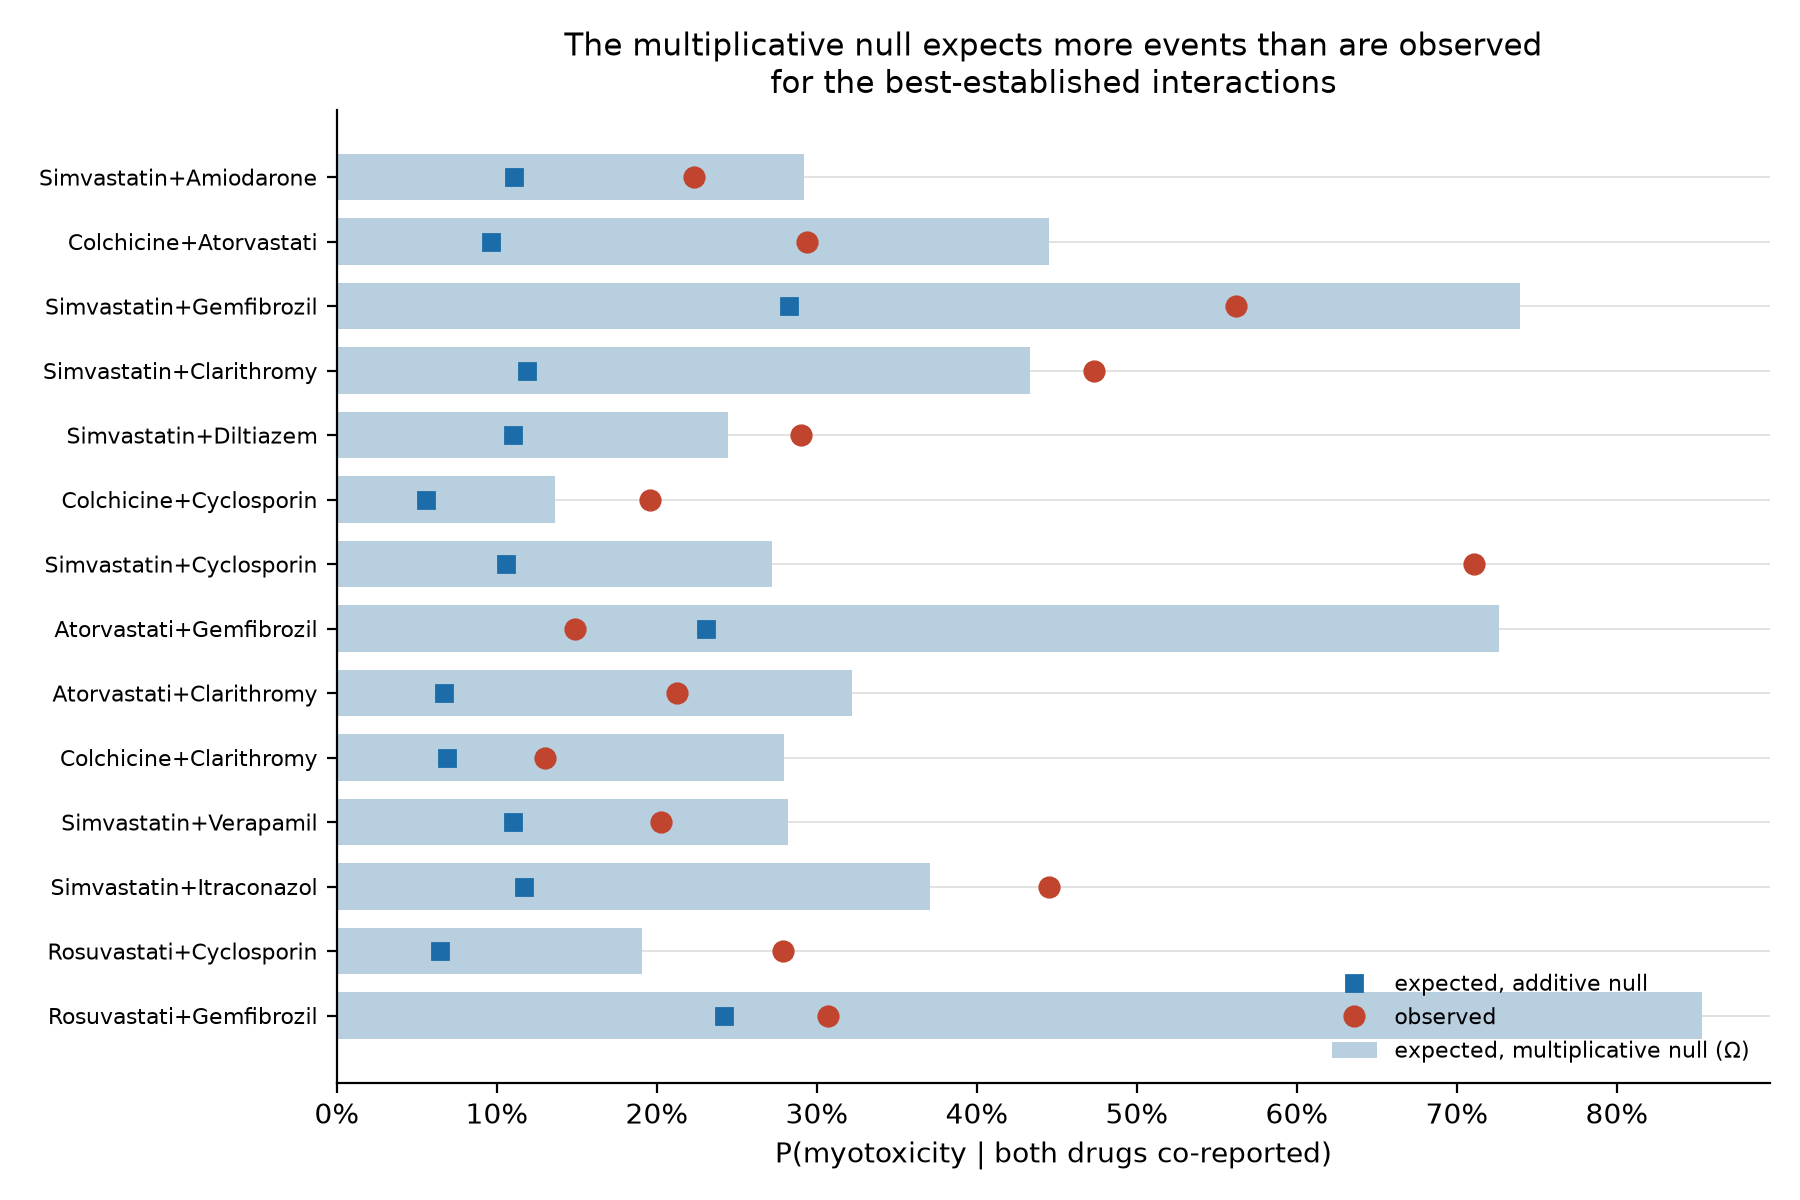
\includegraphics[width=0.85\linewidth]{figure1_null_comparison.png}
\caption{\textbf{Null comparison on positive controls.} Observed proportion of co-reports carrying myotoxicity (red circles) against the proportion expected under the multiplicative null (bars) and the additive null (blue squares), for the 14 controls with at least 50 co-reports.}
\label{fig:1}
\end{figure}

\textbf{The marginal-strength gradient is real but not diagnostic.} Ω correlates with \(\log_2(RR_A \times RR_B)\) at \emph{r} = −0.63 (\emph{n} = 16, 95\% CI −0.86 to −0.19, \emph{p} = 0.009). Because \(E\) is an increasing function of the same marginals that form the x-axis, part of any such correlation is induced by the construction. We measured how much: drawing the triple count from each null's own expectation and recomputing the statistic 10,000 times gives an induced correlation centred on zero (median +0.03, 95\% interval −0.23 to +0.26). The observed −0.63 lies outside it, so the gradient is \textbf{not} an artefact of the estimator.

It is, however, not specific to the multiplicative null (Table 2). \textbf{The observed joint event rate does not rise with marginal strength at all.} Both nulls predict that it should, and steeply; both are wrong in the same direction. The gradient reflects saturation of joint risk in the data rather than a defect peculiar to multiplicativity, and it will appear in any statistic dividing an observed rate by a marginal-driven expectation.

\begin{table}[t]
\centering
\small
\caption{Correlation with \(\log_2(RR_A \times RR_B)\) across the 16 controls.}
\begin{tabular}{@{}
  >{\raggedright\arraybackslash}p{(\linewidth - 4\tabcolsep) * \real{0.3000}}
  >{\raggedright\arraybackslash}p{(\linewidth - 4\tabcolsep) * \real{0.3000}}
  >{\raggedleft\arraybackslash}p{(\linewidth - 4\tabcolsep) * \real{0.4000}}@{}}
\toprule
\begin{minipage}[b]{\linewidth}\raggedright
Quantity
\end{minipage} & \begin{minipage}[b]{\linewidth}\raggedright
\emph{r} (95\% CI)
\end{minipage} & \begin{minipage}[b]{\linewidth}\raggedleft
\emph{p}
\end{minipage} \\
\midrule

\textbf{Observed event rate} & \textbf{+0.12 (−0.40 to +0.58)} & \textbf{0.67} \\
Expected rate, multiplicative & +0.94 & --- \\
Expected rate, additive & +0.94 & --- \\
Ω (multiplicative) & −0.63 (−0.86 to −0.19) & 0.009 \\
\textbf{\(\Omega_{\mathrm{add}}\) (additive)} & \textbf{−0.65 (−0.86 to −0.22)} & \textbf{0.007} \\
\end{tabular}
\end{table}

An earlier version of this work reported this correlation for Ω alone and read it as evidence that the multiplicative null is uniquely broken. That reading was incorrect; it is reported here for both nulls.

What \emph{does} separate them is \textbf{level, not slope}: the multiplicative expectation is far larger at every point (72.9\% versus 27.9\% for gemfibrozil + simvastatin), so the same saturation drives Ω below zero while leaving \(\Omega_{\mathrm{add}}\) above it.

\begin{figure}[htbp]
\centering
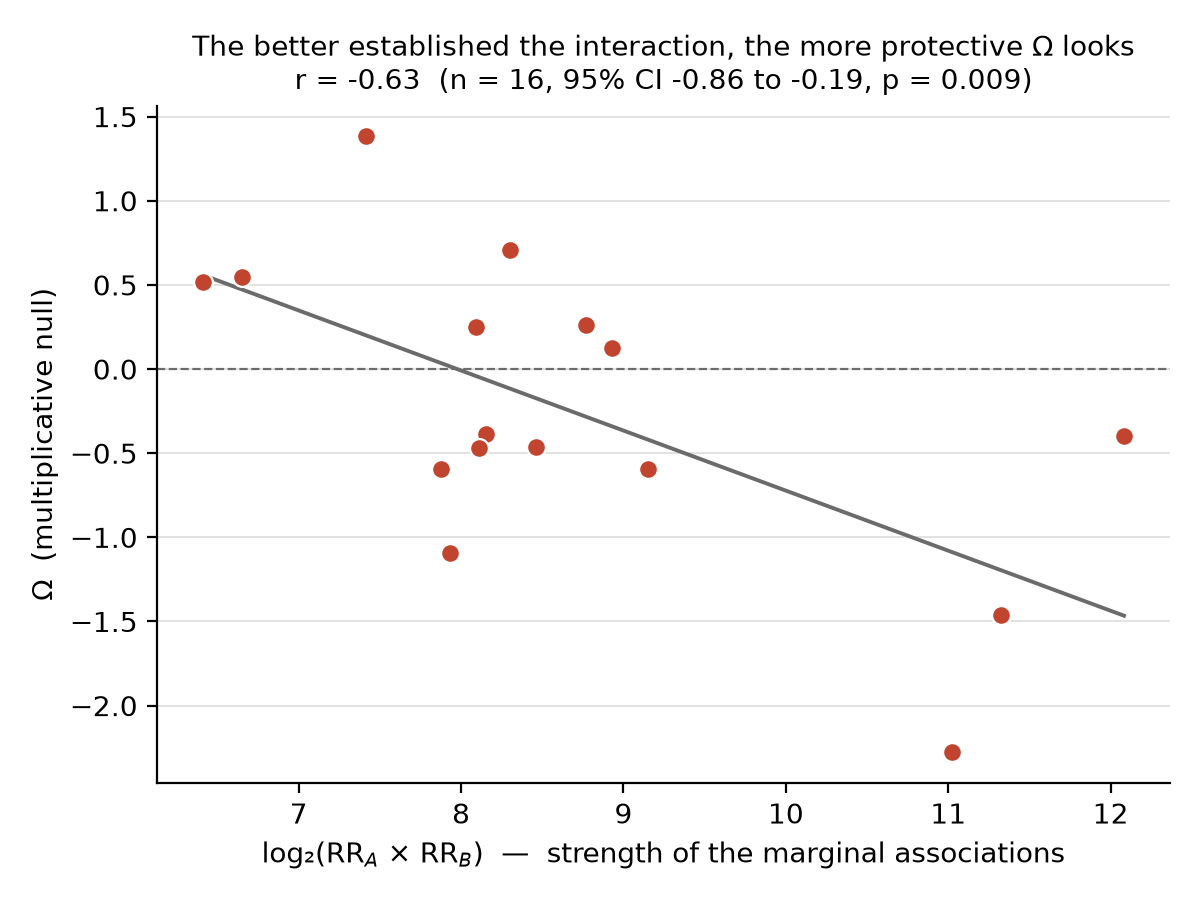
\includegraphics[width=0.85\linewidth]{figure2_omega_correlation.png}
\caption{\textbf{Ω against marginal strength.} Ω for each positive control against $\log_2(RR_A \times RR_B)$. The line is ordinary least squares.}
\label{fig:2}
\end{figure}

\section{5.2 Recovery, calibration and the specification grid}\label{recovery-calibration-and-the-specification-grid}

Under the additive null, 12/16 controls signal (12/14 powered). Because the controls cluster on five victim drugs, the interval must respect that: resampling the victim drug gives \textbf{50--100\%} on the powered subset against a naive binomial 62--97\%, and \textbf{30--96\%} on all 16 against 51--91\%. The naive interval is roughly 40\% too narrow, and we report the clustered one.

\textbf{Pooled false-positive rates, both nulls, both strata.} An earlier version reported the strata for the additive null only, which concealed a sign reversal.

\begin{table}[t]
\centering
\small
\begin{tabular}{@{}lrrrr@{}}
\toprule
stratum & \emph{n} & additive & multiplicative & ratio \\
\midrule

easy (neither drug RR ≥ 2) & 6,674 & 4.02\% & 4.94\% & 0.81 \\
hard (at least one RR ≥ 2) & 9,464 & 8.54\% & 7.50\% & 1.14 \\
\textbf{all} & 16,138 & \textbf{6.67\%} & \textbf{6.44\%} & 1.03 \\
\end{tabular}
\end{table}

The near-identical pooled rates are the average of two differences running in opposite directions. Both exceed the nominal 2.5\%.

\textbf{The negative controls do not occupy the regime the positive controls do.} The generator excludes any pair in which \emph{both} drugs are on the myotoxicity-implicated list --- a reasonable guard against seeding the null set with true positives, but every positive control is exactly such a pair, so the generator cannot produce a negative that resembles a positive. The two populations barely overlap: positive controls sit at a median log₂(RR\_A × RR\_B) of \textbf{8.23} (IQR 7.92--8.99), generated negatives at \textbf{0.56} (IQR −1.52--2.44), and \textbf{only 11 of 16,078 generated negatives (0.1\%) reach the positive controls' interquartile floor}.

Since Section 5.1 establishes that the expected count rises steeply with marginal strength, a rate averaged over that pool is not the rate applying to the pairs being recovered --- and it is not constant across the range. Across quintiles of marginal strength the additive rate runs \textbf{0.93\%, 3.55\%, 7.21\%, 10.86\%, 10.91\%} and the multiplicative \textbf{1.62\%, 5.72\%, 8.64\%, 10.39\%, 5.97\%}: an order of magnitude of variation, and a crossover in the top quintile.

\textbf{A purpose-built negative pool for the regime under study.} Because the standard generator cannot supply one, we built a second pool directly: all pairs among the 1,577 ingredients with RR ≥ 2 and at least 20 co-reports, excluding the positive controls and every pair documented in the endpoint-specific label reference. Pairs in which both drugs are implicated \emph{and} undocumented are also excluded, as too likely to be unrecorded true interactions. Two drugs that each cause an event independently need not interact, so what remains is a legitimate negative set --- 19,826 pairs, median strength 4.31.

Across the whole purpose-built pool the additive null fires on 7.2\% and the multiplicative on 3.7\%. \textbf{Restricted to the 2,345 pairs at positive-control strength, the rates are 9.3\% and 2.2\%} --- against 9.0\% and 1.2\% on the 166 in-regime pairs the standard generator happens to yield. The two pools agree, and the purpose-built one carries fourteen times the sample. \textbf{Against a nominal 2.5\%, Ω is about twice as conservative as advertised in this regime and Ω\_add about four times too permissive.}

\textbf{Recovery at matched in-regime error rates.} Calibrating each null against the in-regime negatives separates the choice of null from the choice of operating point:

\begin{table}[t]
\centering
\small
\begin{tabular}{@{}
  >{\raggedright\arraybackslash}p{(\linewidth - 6\tabcolsep) * \real{0.2000}}
  >{\raggedleft\arraybackslash}p{(\linewidth - 6\tabcolsep) * \real{0.2667}}
  >{\raggedleft\arraybackslash}p{(\linewidth - 6\tabcolsep) * \real{0.2667}}
  >{\raggedleft\arraybackslash}p{(\linewidth - 6\tabcolsep) * \real{0.2667}}@{}}
\toprule
\begin{minipage}[b]{\linewidth}\raggedright
operating point
\end{minipage} & \begin{minipage}[b]{\linewidth}\raggedleft
additive
\end{minipage} & \begin{minipage}[b]{\linewidth}\raggedleft
multiplicative
\end{minipage} & \begin{minipage}[b]{\linewidth}\raggedleft
gap
\end{minipage} \\
\midrule

\(\Omega_{025}\) \textgreater{} 0 (as published) & 12/16 @ 9.0\% & 4/16 @ 1.2\% & \textbf{8} \\
matched at 5\% in-regime FPR & 12/16 & 10/16 & \textbf{2} \\
matched at 10\% & 12/16 & 11/16 & \textbf{1} \\
matched at 20\% & 14/16 & 12/16 & \textbf{2} \\
\end{tabular}
\end{table}

\textbf{The eight-pair gap becomes one to two once error rates are equalised.} The additive null still wins at every matched rate, so the direction is real, but most of the apparent advantage comes from the conventional threshold being far more permissive for Ω\_add than for Ω here: the multiplicative null must move to about −1.4 to reach 9\% in-regime, precisely because Ω is systematically negative in this regime (Section 5.1).

\emph{Caveat.} The matched-rate calibration rests on the 166 in-regime pairs of the generated pool, so the 5\%/10\%/20\% points sit on roughly 8/17/33 of them and are noisy. The purpose-built pool confirms the rates at 2,345 pairs but the matched-recovery table has not been recomputed on it, and the in-regime cut --- the marginal strength of the weakest positive control --- is our choice rather than pre-specified.

A quantile of the pool whose false-positive rate is then reported returns its target by construction. Splitting the pool 500 times --- calibrating on one half, measuring on the other --- gives a held-out threshold of +0.429 and a held-out false-positive rate of \textbf{5.03\% (95\% CI 4.37--5.74\%)} against the in-sample +0.436. The in-sample calibration is therefore very nearly unbiased, but the rate is now a measurement.

\textbf{All four design arms are reported} (Table 3). Two binary choices were available: the event tier (\texttt{core}, specific; \texttt{broad}, inclusive of the two non-meaning-preserving concepts) and the drug role policy (\texttt{primary}, suspect roles only; \texttt{sensitivity}, wider). \texttt{core}/\texttt{primary} is pre-specified in configuration and is the arm reported throughout.

\begin{table}[t]
\centering
\small
\caption{Positive-control recovery across all four specifications.}
\begin{tabular}{@{}
  >{\raggedright\arraybackslash}p{(\linewidth - 8\tabcolsep) * \real{0.1667}}
  >{\raggedright\arraybackslash}p{(\linewidth - 8\tabcolsep) * \real{0.1667}}
  >{\raggedleft\arraybackslash}p{(\linewidth - 8\tabcolsep) * \real{0.2222}}
  >{\raggedleft\arraybackslash}p{(\linewidth - 8\tabcolsep) * \real{0.2222}}
  >{\raggedleft\arraybackslash}p{(\linewidth - 8\tabcolsep) * \real{0.2222}}@{}}
\toprule
\begin{minipage}[b]{\linewidth}\raggedright
Tier
\end{minipage} & \begin{minipage}[b]{\linewidth}\raggedright
Role policy
\end{minipage} & \begin{minipage}[b]{\linewidth}\raggedleft
Additive
\end{minipage} & \begin{minipage}[b]{\linewidth}\raggedleft
Multiplicative
\end{minipage} & \begin{minipage}[b]{\linewidth}\raggedleft
Advantage
\end{minipage} \\
\midrule

\textbf{core} & \textbf{primary} \emph{(pre-specified)} & \textbf{12/16} & \textbf{4/16} & \textbf{+8} \\
core & sensitivity & 12/16 & 4/16 & +8 \\
broad & primary & 11/16 & 4/16 & +7 \\
\textbf{broad} & \textbf{sensitivity} & \textbf{6/16} & \textbf{6/16} & \textbf{0} \\
\end{tabular}
\end{table}

\textbf{Under the widest event definition combined with the widest role policy, the additive advantage disappears entirely.} The contrast holds in three of four arms and is null in the fourth. It is robust to either widening alone, not to both together. The fourth arm is the least specific analysis available, but it is not unreasonable, and it is on the record.

\section{5.3 Polypharmacy leverage}\label{polypharmacy-leverage}

The strongest apparent false positive was alirocumab + ipratropium: 88 co-reports, 88 events. Those 88 cases share 5 distinct event dates and 1 distinct age, each listing 31--40 drugs --- residual near-duplicates the exact-set fingerprint could not merge.

A case listing 40 drugs contributes 780 pairs. \textbf{19,005 cases (0.09\% of the database) contribute 34.7\% of all drug pairs at a 4× enriched event rate.} Capping at 20 drugs per case improved sensitivity (11 → 12/16) and the false-positive rate (6.9\% → 6.7\%) simultaneously, and the multiplicative null improves from 2/16 to 4/16, so the contrast in Section 5.1 is \emph{understated} by the cap rather than produced by it.

Nothing in the positive controls could have revealed this: it is visible only from the false-positive side, which has a direct consequence for how such screens should be validated. The cap \emph{value}, however, was chosen by looking at control recovery. Table 4 reports the full sweep: capping is justified at every value, the conclusion is flat from 15 to 40, and a cap of 10 would have been better on both axes.

\begin{table}[t]
\centering
\small
\caption{Polypharmacy cap sweep.}
\begin{tabular}{@{}rrrrr@{}}
\toprule
Cap & Analysis cases & Additive & Multiplicative & FPR \\
\midrule

10 & 20,202,853 & \textbf{13/16} & 4/16 & \textbf{6.0\%} \\
15 & 20,259,682 & 12/16 & 4/16 & 6.0\% \\
\textbf{20 (adopted)} & 20,274,416 & 12/16 & 4/16 & 6.7\% \\
30 & 20,284,277 & 12/16 & 2/16 & 7.8\% \\
40 & 20,288,002 & 12/16 & 2/16 & 7.6\% \\
None & 20,293,421 & 11/16 & 2/16 & 6.9\% \\
\end{tabular}
\end{table}

\begin{figure}[htbp]
\centering
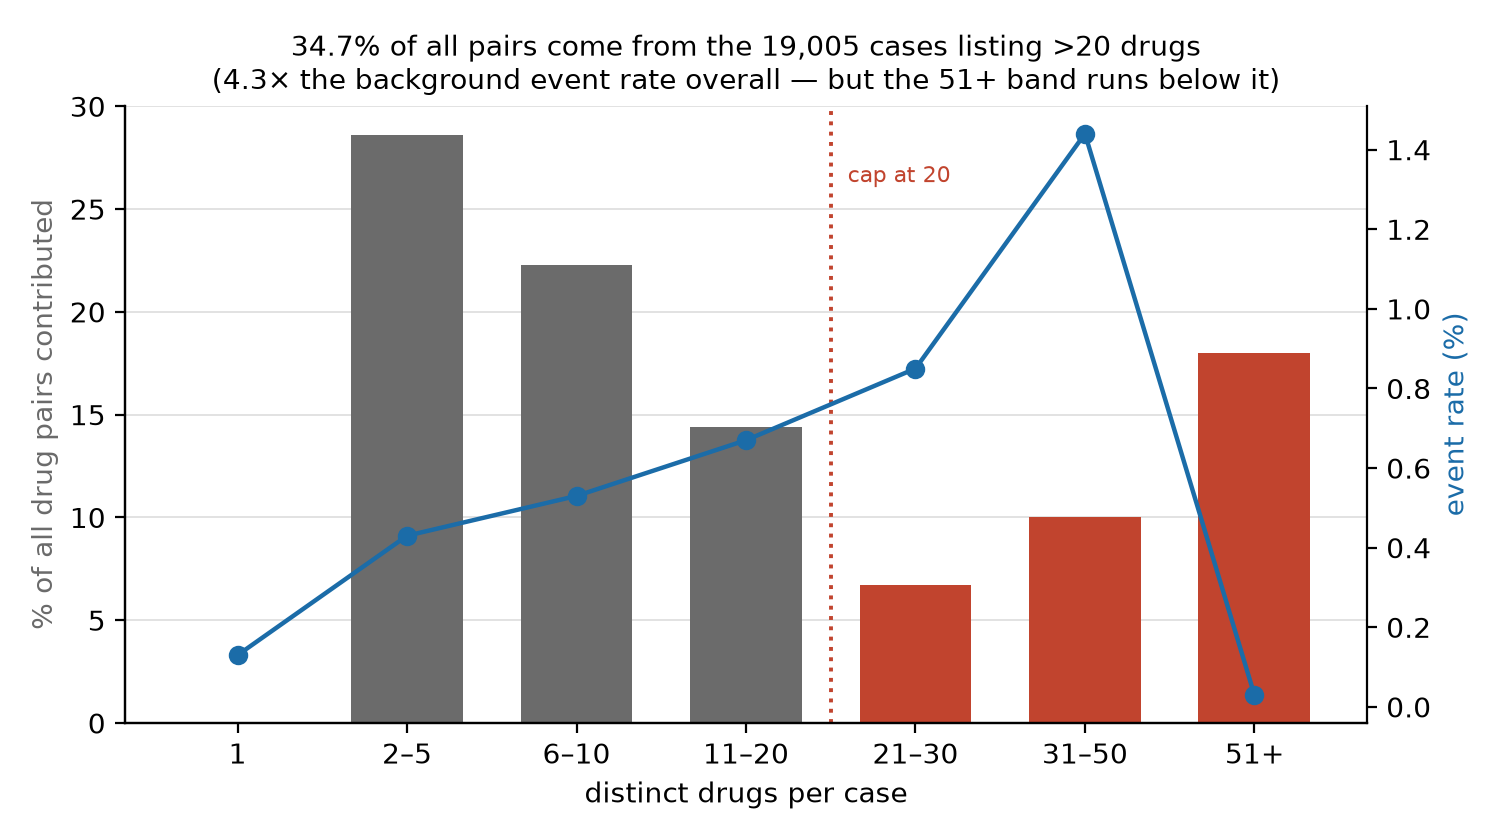
\includegraphics[width=0.85\linewidth]{figure5_polypharmacy_leverage.png}
\caption{\textbf{Polypharmacy leverage.} Percentage of all drug pairs contributed by cases in each drugs-per-case band (bars, left axis) and the myotoxicity event rate within that band (line, right axis). The dotted line marks the adopted cap.}
\label{fig:3}
\end{figure}

\section{5.4 The estimand switch does not inflate sensitivity}\label{the-estimand-switch-does-not-inflate-sensitivity}

The additive null was adopted because it recovered more controls at the conventional threshold --- selection on the evaluation set. The decision is binary and was cross-validated: the additive null wins in \textbf{16/16 leave-one-out folds}. That establishes only that the choice does not hinge on any single control; when one null wins every fold, held-out recovery equals in-sample recovery by construction, so the optimism of 0.000 is a consequence of stability rather than evidence for it. Section 5.2 supersedes this analysis in any case: once error rates are matched the choice between nulls is worth one to two pairs, so what it was cross-validating barely matters.

It does not address the choice of \emph{controls}. A second set was therefore drawn by FDA labelling rather than by us --- every label-documented myotoxicity pair with at least 50 co-reports not among the 16 (Table 5). The direction replicates at both operating points, but the recovery \emph{rate} collapses from 86\% to 12--16\%.

\begin{table}[t]
\centering
\small
\caption{Recovery on author-selected and label-selected controls.}
\begin{tabular}{@{}
  >{\raggedright\arraybackslash}p{(\linewidth - 8\tabcolsep) * \real{0.1667}}
  >{\raggedleft\arraybackslash}p{(\linewidth - 8\tabcolsep) * \real{0.2222}}
  >{\raggedright\arraybackslash}p{(\linewidth - 8\tabcolsep) * \real{0.1667}}
  >{\raggedleft\arraybackslash}p{(\linewidth - 8\tabcolsep) * \real{0.2222}}
  >{\raggedleft\arraybackslash}p{(\linewidth - 8\tabcolsep) * \real{0.2222}}@{}}
\toprule
\begin{minipage}[b]{\linewidth}\raggedright
Control set
\end{minipage} & \begin{minipage}[b]{\linewidth}\raggedleft
\emph{n}
\end{minipage} & \begin{minipage}[b]{\linewidth}\raggedright
Threshold
\end{minipage} & \begin{minipage}[b]{\linewidth}\raggedleft
Mult.
\end{minipage} & \begin{minipage}[b]{\linewidth}\raggedleft
Additive
\end{minipage} \\
\midrule

Author-selected, all & 16 & \(\Omega_{025}\) \textgreater{} 0 & 4/16 & \textbf{12/16} \\
Author-selected, powered & 14 & \(\Omega_{025}\) \textgreater{} 0 & 4/14 & \textbf{12/14} \\
Label-selected & 349 & \(\Omega_{025}\) \textgreater{} 0 & 29/349 & \textbf{55/349} \\
Label-selected & 349 & +0.436 & 15/349 & \textbf{42/349} \\
\end{tabular}
\end{table}

Every cell carries its own denominator; an earlier version reported the author-selected row with \emph{n} = 14 while giving the multiplicative count out of 16.

\textbf{That gap is not statistical power.} Co-report counts are indistinguishable between the sets (median 420 versus 321, Mann--Whitney \emph{p} = 0.45), and recovery in the label-selected set \emph{falls} as co-reporting rises --- 19\%, 17\%, 10\%, 2\%, 0\% across quartiles and the top decile. The mechanism is the event rate among co-reports: 29.2\% for author-selected pairs (141.4× baseline) against 0.72\% for label-selected (3.5×), and 0.12\% for the top decile (\textbf{0.57×}, below baseline). The most heavily co-reported label-documented pairs show no elevation at all; they are common co-prescriptions carrying a \emph{class} warning rather than a pair-specific one. Neither figure is the method's sensitivity --- 86\% is an upper bound contaminated by selection for famous interactions, 12\% a lower bound contaminated by pairs with no detectable signal. They bracket it.

A further reason not to read 12\% as the sensitivity: the label-selected control set is drawn from FDA product labelling, and that reference is \textbf{structurally blind to 11 of the 200 screened ingredients (5.5\%)} --- because no label exists for them at all. Those 11 are well co-reported, so they account for \textbf{9.8\% of screened pairs}. The gap falls on agents without a current US marketing authorisation, and the one that matters here is \textbf{fusidic acid}, whose statin combination is contraindicated in practice. Any control set drawn from that reference is incomplete in a way that correlates with the outcome. The companion paper quantifies the effect on measured enrichment; here it bounds how tightly the lower end of the bracket can be trusted.

\section{5.5 Replication on a second drug-dominant event}\label{replication-on-a-second-drug-dominant-event}

One event demonstrates the phenomenon, not the condition. Two further events were analysed (Table 6). The torsade PT list is curated to the same standard as the primary event --- repolarisation-specific terms only. An earlier version also counted non-specific terminal events, tripling the event rate and making the replication a looser test than the analysis it replicated; both lists are reported.

\begin{table}[t]
\centering
\small
\caption{Recovery and gradient across events.}
\begin{tabular}{@{}
  >{\raggedright\arraybackslash}p{(\linewidth - 10\tabcolsep) * \real{0.1429}}
  >{\raggedleft\arraybackslash}p{(\linewidth - 10\tabcolsep) * \real{0.1905}}
  >{\raggedleft\arraybackslash}p{(\linewidth - 10\tabcolsep) * \real{0.1905}}
  >{\raggedleft\arraybackslash}p{(\linewidth - 10\tabcolsep) * \real{0.1905}}
  >{\raggedright\arraybackslash}p{(\linewidth - 10\tabcolsep) * \real{0.1429}}
  >{\raggedright\arraybackslash}p{(\linewidth - 10\tabcolsep) * \real{0.1429}}@{}}
\toprule
\begin{minipage}[b]{\linewidth}\raggedright
Event
\end{minipage} & \begin{minipage}[b]{\linewidth}\raggedleft
Rate
\end{minipage} & \begin{minipage}[b]{\linewidth}\raggedleft
Mult.
\end{minipage} & \begin{minipage}[b]{\linewidth}\raggedleft
Additive
\end{minipage} & \begin{minipage}[b]{\linewidth}\raggedright
Ω gradient
\end{minipage} & \begin{minipage}[b]{\linewidth}\raggedright
\(\Omega_{\mathrm{add}}\) gradient
\end{minipage} \\
\midrule

Rhabdomyolysis & 0.207\% & 4/16 & 12/16 & −0.63 (\emph{p} = 0.009) & −0.65 (\emph{p} = 0.007) \\
\textbf{Torsade (curated)} & 0.199\% & \textbf{0/10} & \textbf{9/10} & \textbf{−0.81 (\emph{p} = 0.005)} & −0.79 (\emph{p} = 0.006) \\
Torsade (broad) & 0.659\% & 1/10 & 7/10 & −0.76 (\emph{p} = 0.011) & −0.72 (\emph{p} = 0.020) \\
Anaphylaxis & 0.410\% & 1/4 & 1/4 & \emph{n} = 4 & \emph{n} = 4 \\
\end{tabular}
\end{table}

At \(\Omega_{025}\) \textgreater{} 0, Ω recovers 0/10 on torsade against 9/10 for the additive null --- an apparently stronger version of the primary result on an independent event whose rate is within 4\% of it. Amiodarone + sotalol, two of the most strongly QT-prolonging agents in use, scores Ω = −1.63, and the marginal-strength gradient reproduces under both nulls.

\textbf{That apparent replication does not survive matched error rates, and we report it as a failed replication.} Applying Section 5.2's analysis to torsade, the in-regime false-positive rates at \(\Omega_{025}\) \textgreater{} 0 are \textbf{2.0\% for Ω and 42.8\% for the additive null} --- the additive null fires on nearly half of strongly-associated non-interacting pairs. Recalibrating both to a common in-regime rate:

\begin{table}[t]
\centering
\small
\caption{Torsade recovery at matched in-regime error rates (152 in-regime negatives).}
\begin{tabular}{@{}lrr@{}}
\toprule
operating point & additive & multiplicative \\
\midrule

\(\Omega_{025}\) \textgreater{} 0 (as published) & 9/10 @ 42.8\% & 0/10 @ 2.0\% \\
matched at 5\% in-regime FPR & \textbf{0/10} & \textbf{0/10} \\
matched at 10\% & \textbf{1/10} & \textbf{1/10} \\
matched at 20\% & \textbf{4/10} & \textbf{3/10} \\
\end{tabular}
\end{table}

\textbf{At any common error rate neither null recovers these pairs, and the additive null has no advantage.} The 9-versus-0 result is an artefact of the conventional threshold sitting at wildly different error rates for the two measures on this event.

What replicates on torsade is therefore the \emph{calibration} finding, not the recovery finding: Ω is again far more conservative than its nominal 2.5\% (2.0\%) and the additive null far more permissive (42.8\%), by a wider margin than on rhabdomyolysis. What does \textbf{not} replicate is that the additive null recovers more at a common error rate. On the primary event it retains a one-to-two-pair advantage; here it retains none.

We report this because we ran the check, not because a reviewer asked for it, and it is the reason this paper's claim is about calibration rather than about which null is better.

\textbf{The anaphylaxis arm is invalid by construction, not underpowered.} It was intended as the negative case --- an event with diffuse marginals where Ω should do comparatively well --- but anaphylaxis is essentially single-agent, and there is no established pair whose \emph{interaction} causes it. The pairs available are co-exposures among independently causative agents. There is nothing for either null to detect, so no additional data would make the arm informative. The calibration finding therefore generalises to a second event; the recovery advantage does not, and the conditional claim about \emph{why} the nulls misbehave has no valid negative case and remains a hypothesis.

\section{5.6 Sensitivity to the shrinkage constant}\label{sensitivity-to-the-shrinkage-constant}

α = 0.5 is conventional and could not be verified against the primary source. Varying it over a 20-fold range and recalibrating at each value, control recovery varies by two pairs (10/15 to 12/15) and the signal count by 7\% (998 to 1,069). No conclusion turns on α.

\section{6. Discussion}\label{discussion}

\textbf{Neither null is usable at its conventional threshold for drug-dominant events.} Against a nominal 2.5\%, \(\Omega_{025}\) \textgreater{} 0 fires on 2.2\% of strongly-associated non-interacting pairs on the primary event and 2.0\% on the replication --- roughly as advertised, but paired with near-zero sensitivity because Ω is systematically negative in this regime. \(\Omega_{\mathrm{add},025}\) \textgreater{} 0 fires on 9.3\% and 42.8\% --- four- to seventeen-fold too permissive. This is precisely the situation for the best-characterised interaction classes, which is where a DDI method is most likely to be validated, so it is a failure mode a method could pass into routine use without encountering. A method calibrated on conventionally generated negative controls will not detect it, because those controls exclude the pair configuration every positive control has.

\textbf{The apparent superiority of the additive null is mostly an operating-point effect.} At matched in-regime error rates the eight-pair advantage on rhabdomyolysis becomes one to two pairs, and on torsade it disappears entirely. An earlier version of this work reported the unmatched comparison as its primary evidence. It is not, and that correction is why this paper's claim is now about calibration rather than about which null to prefer.

The recommendation is checkable in advance at essentially no cost: \textbf{compute the marginal relative risks first, then calibrate the threshold against negative controls drawn from the same regime.} Neither the choice of null nor a nominal credibility bound substitutes for that.

\textbf{The mechanism is narrower than we first claimed.} Observed joint rates are flat in marginal strength while both nulls predict them to rise steeply. Joint risk saturates and both models miss it; the multiplicative null fails much harder only because its expectation is larger everywhere. We initially read the Ω-versus-marginals correlation as diagnostic of multiplicativity. It is not; both nulls show it. Nor, as it turns out, is the recovery comparison diagnostic unless the error rates are matched first.

\textbf{Deployment.} The two nulls must be compared at matched false-positive rates rather than at a common nominal cut, and the negative-control pool used for calibration must contain pairs resembling those the system will be asked to judge. A pooled 6.7\% against a nominal 2.5\% already shows how far a nominal threshold drifts; the in-regime 9.3\% and 42.8\% show that the pooled figure is itself optimistic. Alert burden is the practical cost: a surveillance system adopting the additive null on the strength of the unmatched comparison would run at roughly nine percent false positives among strongly-associated pairs, not the one to two percent Ω delivers there. Compute is not the constraint --- the full history fits on one workstation and the analysis completes in minutes.

\textbf{Polypharmacy leverage} is a property of pairwise combinatorics rather than of any endpoint, and generalises directly. Any pairwise screen over spontaneous reports should cap drugs per case and report the cap with its sensitivity.

\section{7. Limitations}\label{limitations}

The 16 positive controls are author-selected, are the only positive evaluation set, and comprise five victim drugs rather than sixteen independent trials; intervals are widened accordingly (50--100\%). Leave-one-out addresses optimism in estimand choice only.

The headline contrast is \textbf{not robust to widening both design choices at once} (Table 3, fourth arm).

The conditional claim is not established: the intended negative case was invalid rather than underpowered, and constructing a valid one requires an event with weak marginals \emph{and} documented interacting pairs --- a combination we could not find.

\textbf{The in-regime error rates rest on constructed negative controls, and the matched-recovery table on a small subset of them.} The purpose-built pool (19,826 pairs, 2,345 in regime) excludes documented interactions, so any undocumented true interaction it contains inflates the measured false-positive rate; every rate here is an upper bound, as with any spontaneous-reporting negative control set. The matched-recovery calibration uses the 166 in-regime pairs of the generated pool and is noisy at the tails; it has not been recomputed on the larger pool. The in-regime cut is the marginal strength of the weakest positive control, which is our choice and not pre-specified.

\textbf{The recovery advantage of the additive null is one to two pairs on 16 controls.} With five victim-drug clusters and a 50--100\% interval on the unmatched estimate, a one-to-two-pair difference is not separable from noise, and we do not claim it is. What the data support is the calibration finding, not a ranking of the two nulls.

Ingredient resolution accuracy is bounded, not directly measured: FDA's own annotation of a given verbatim name is 98.99\% self-consistent, which bounds the backfill, but no manual audit against external ground truth was performed. The PT list had a single curator. The near-duplicate rule uses exact set matching, and the residual is bounded at 226 cases (1.17\% of event cases). α = 0.5 is corroborated by secondary sources only; the primary paper is paywalled and unread by the authors.

No external reporting system was used. Two pipeline components are externally benchmarked --- deduplication against AEOLUS (8\% apart) and ingredient resolution against DiAna (98.0\% versus 98.94\%) --- and the central finding replicates on a second event within FAERS, but conclusions may be FAERS-specific. Spontaneous reporting has no exposure denominator: nothing here estimates risk, only reporting disproportionality.

The evaluation of this pipeline as a \emph{discovery} instrument, and the reference-quality problems that bound it, are reported separately in a companion paper.

\section{8. Conclusion}\label{conclusion}

The conventional operating points of both disproportionality nulls are severely miscalibrated when the drugs under study are the dominant reported causes of the outcome. Measured against a purpose-built pool of 2,345 strongly-associated non-interacting pairs, \(\Omega_{025}\) \textgreater{} 0 fires on 2.2\% and \(\Omega_{\mathrm{add},025}\) \textgreater{} 0 on 9.3\%, against a nominal 2.5\% for both; on a second event the additive figure is 42.8\%. Conventionally generated negative controls cannot reveal this, because they exclude the pair configuration every positive control has and sit two orders of magnitude away in marginal strength.

The recovery comparison that motivated this work is largely an artefact of that miscalibration: an eight-pair advantage for the additive null at the conventional threshold becomes one to two pairs at matched error rates on the primary event, and none on the replication. The mechanism is that observed joint risk saturates while both nulls predict it to rise with marginal strength, so the two differ in the level of their expectation rather than its gradient --- which is why the gradient alone does not identify which null is at fault, and why the useful question is not which null to choose but where to put the threshold.

Separately, high-polypharmacy reports exert leverage far out of proportion to their number: 0.09\% of cases contribute 34.7\% of all drug pairs at a 4× enriched event rate, invisible from positive controls and detectable only from the false-positive side.

Both findings are checkable before analysis and cost nothing to act on.

\section{Computational environment and reproducibility}\label{computational-environment-and-reproducibility}

A single workstation, macOS on Apple silicon; Python 3.14.6, DuckDB 1.5.5, pandas 3.0.5, PyArrow 25.0.0, NumPy 2.5.1, SciPy 1.18.0, matplotlib. Exact pinned versions accompany the code. Downloading the 90 archives takes roughly 30 minutes on a domestic connection, parsing 328,476,258 rows to Parquet about 3 minutes at 4 processes, and the full analysis about 12 minutes. Peak memory is bounded by a 10 GB DuckDB limit; no GPU is used.

Every stochastic procedure is seeded and the seeds are in the shipped configuration: the drug-level cluster bootstrap (20,000 draws for control recovery, 1,000 for enrichment intervals), the drug-level permutation test (10,000 permutations), the induced-correlation simulation (10,000 draws) and the 500-split threshold calibration. The pipeline is deterministic: two full runs produce byte-identical output, and this is checked rather than asserted.

\section{Data and code availability}\label{data-and-code-availability}

All code, configuration and result tables are available at
\url{https://github.com/edanmn/faers-ddi-rhabdomyolysis}. Every figure quoted in the Abstract and Results is generated into \texttt{results/canonical\_numbers.json} by a single deterministic run and asserted against this text by \texttt{tests/test\_canonical\_numbers.py}; pipeline statistics quoted in Methods are persisted under \texttt{audit.provenance} in the same file and asserted alongside them. Figures drawn from cited work are attributed and not regenerated. The pipeline is deterministic: two full runs produce byte-identical output.

\textbf{This is research code and a research result. It is not clinical guidance.}

\section{Acknowledgements}\label{acknowledgements}

{[}TODO{]}

\clearpage
\label{sec:endofbody}
\section{References}\label{references}

\begin{enumerate}
\def\labelenumi{\arabic{enumi}.}
\tightlist
\item
  Bate A, Lindquist M, Edwards IR, Olsson S, Orre R, et al.~A Bayesian neural network method for adverse drug reaction signal generation. \emph{Eur J Clin Pharmacol.} 1998;54(4):315--321. doi:10.1007/s002280050466
\item
  Banda JM, Evans L, Vanguri RS, Tatonetti NP, Ryan PB, Shah NH. A curated and standardized adverse drug event resource to accelerate drug safety research. \emph{Sci Data.} 2016. PMID 27193236.
\item
  DuMouchel W. Bayesian data mining in large frequency tables, with an application to the FDA spontaneous reporting system. \emph{Am Stat.} 1999;53(3):177--190. doi:10.1080/00031305.1999.10474456
\item
  Evans SJW, Waller PC, Davis S. Use of proportional reporting ratios (PRRs) for signal generation from spontaneous adverse drug reaction reports. \emph{Pharmacoepidemiol Drug Saf.} 2001;10(6):483--486. doi:10.1002/pds.677
\item
  Fusaroli M, et al.~Enhancing transparency in defining studied drugs: the open-source living DiAna dictionary for standardizing drug names in the FAERS. \emph{Drug Saf.} 2024;47:271--284.
\item
  Norén GN, Sundberg R, Bate A, Edwards IR. A statistical methodology for drug--drug interaction surveillance. \emph{Stat Med.} 2008;27(16):3057--3070. PMID 18344185. doi:10.1002/sim.3247
\item
  Rothman KJ. Causes. \emph{Am J Epidemiol.} 1976;104(6):587--592.
\item
  Thakrar BT, Grundschober SB, Doessegger L. Detecting signals of drug--drug interactions in a spontaneous reports database. \emph{Br J Clin Pharmacol.} 2007;64(4):489--495.
\item
  VanderWeele TJ, Knol MJ. A tutorial on interaction. \emph{Epidemiol Methods.} 2014;3(1):33--72. doi:10.1515/em-2013-0005
\end{enumerate}


\end{document}
